\documentclass[12pt,letterpaper]{article}


\newcommand{\studentname}{Ben Bassett}
% \newcommand{\labpartner}{Katrina Sumarli}

\title{\textsc{Lab 06: The RL Circuit}}
\newcommand{\shorttitle}{The RL Ciruit}

\newcommand{\course}{PHY310}
\newcommand{\labdate}{10-15-2024}

%------------------------------------------------------------------------------------------------------------

\usepackage[letterpaper,left=1in,right=1in,bottom=1in,top=1in]{geometry}
\usepackage{fancyhdr}
\usepackage{subfigure}
\usepackage{graphicx}
\usepackage{amsmath}
\usepackage{cleveref}
\usepackage{booktabs}
\usepackage[british]{babel}
\usepackage[square,comma,numbers,sort&compress]{natbib}
\usepackage{csvsimple}
\usepackage{graphicx}
\usepackage{pgfplotstable}
\usepackage{textcomp,gensymb}
\usepackage{array}
\usepackage{tabu}
\usepackage{multirow}
\usepackage{url}
\usepackage{lipsum}
\usepackage{dsfont}
\pgfplotsset{compat=1.9}% supress warning
\begin{document}

%------------------------------------------------------------------------------------------------------------

\setlength{\parindent}{1em}
\setlength{\parskip}{0.5em}
\author{\course~Lab Journal \\ \\ \studentname} % \,\& \labpartner}
\date{\labdate}

\renewcommand\abstractname{Summary}

\pagestyle{fancy}
\fancyhead{}
\fancyhead[l]{\course:~\shorttitle}
\fancyhead[r]{\studentname}
\fancyfoot{}
\fancyfoot[C]{\thepage}
\renewcommand{\headrulewidth}{0pt}
\renewcommand{\footrulewidth}{0pt}

\renewcommand\bibname{References}

%------------------------------------------------------------------------------------------------------------

\renewcommand\abstractname{Abstract}
\maketitle

% COMMENT IN IF ASKED TO SUBMIT REPORT WITH ABSTRACT
%\begin{abstract}
%Maximum 200 words.
%\end{abstract}

\section{Purpose}
This lab aimed to measure the self-inductance of the Helmholtz coils using an RL circuit.

\section{Experimental Apparatus}

Materials given were a Helmholtz coil, variable resistor, a voltmeter and ammeter, a function generator, and various cables. My general setup is illustrated in Figure \ref{fig:setup}.

\begin{figure}[h]
    \centering
    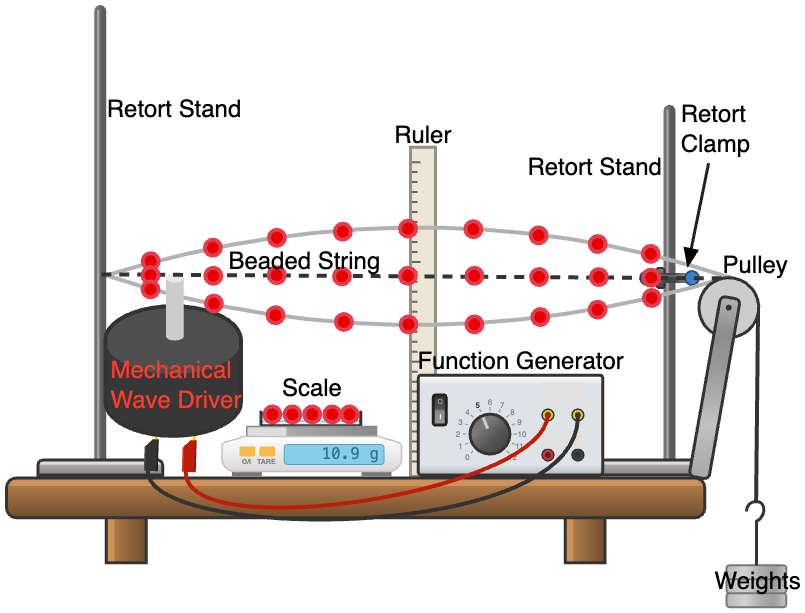
\includegraphics[width=6in]{images/setup.png}
    \caption{A diagram of my experimental setup}
    \label{fig:setup}
\end{figure}

% \pagebreak
\section{Procedure}

To measure the self-inductance of the coil, I first set the variable resistor to 20 Ohms, then placed it in series with the coil and measured the resistance of the entire circuit and the coil alone. I attached the resistor and inductor in series to the function generator, but put an ammeter between the function generator and the resistor, and a voltmeter/voltage probes across the resistor and across the coil/inductor.

I began by using a sinusoidal wave on the function generator to observe the phase of the voltage in the circuit. I did this at 10 and 100 Hz, but after less success at 100 Hz decided to stick to 10 Hz. I then switched to using a square wave at 10 Hz, and recorded a variety of sensor configurations in this setup. The function generator was set at 4 volts the entire time.

\section{Results}

I measured the resistance of the entire circuit to be 26.3 Ohms, and the resistance of the Helmholtz coil alone to be 3.7 Ohms. Let's write this as an equation.

\begin{align*}
    R_{\text{total}}&=R_{\text{coil}}+R_{\text{resistor}} \\
    26.3 \, \Omega &= 3.7 \, \Omega + 22.6 \, \Omega
\end{align*}

Slightly disturbing that the supposed 20 Ohm resistor is in reality 2.6 Ohms off, but we'll accept it as long as we know what it is.

While the measurement of inductance should be independent of the measurement we used, it's just easier to see at smaller frequencies, which is why I picked 10. While I had a wealth of data to choose from, I just grabbed the first third of a second of the 10 Hz square wave, since it seemed visually the same as the other 17 seconds of data. See the current, inductor voltage, and resistor voltage graphed in Figure \ref{fig:square}.

\begin{figure}[ht]
    \centering
    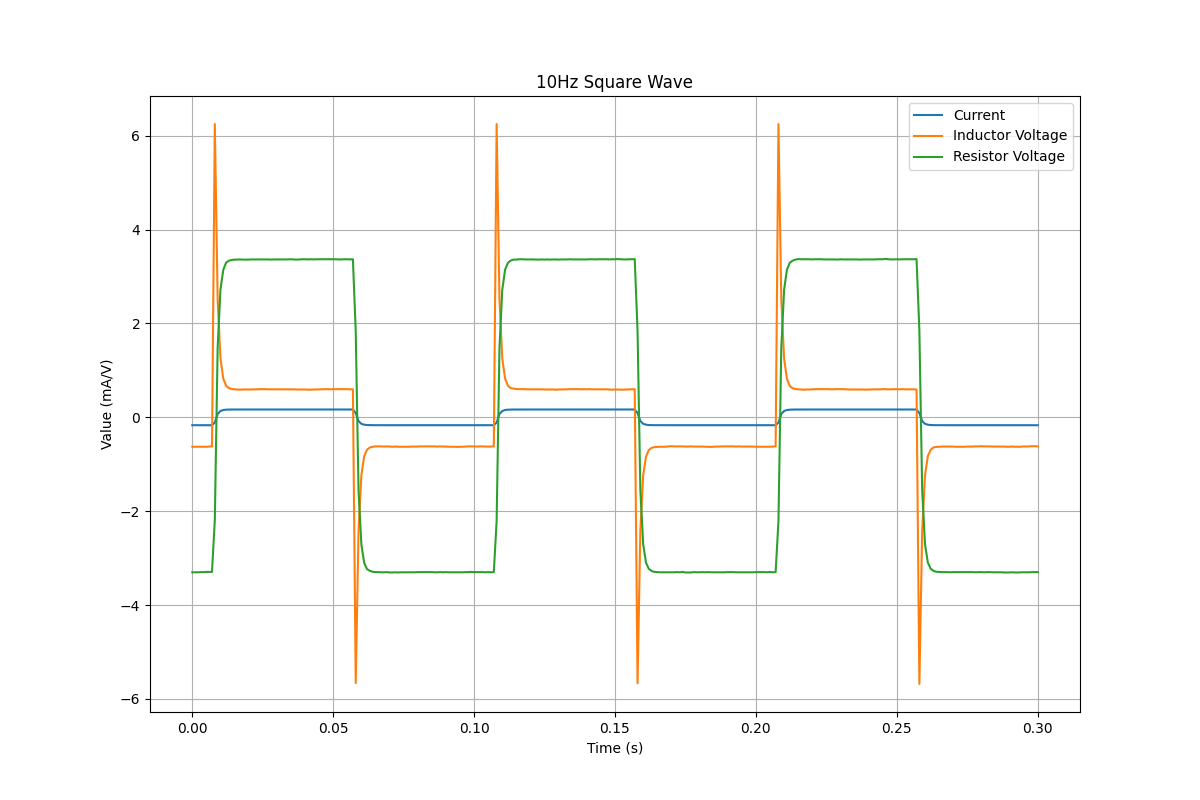
\includegraphics[width=5in]{images/all-square.png}
    \caption{Current, inductor voltage, and resistor voltage w.r.t. time}
    \label{fig:square}
\end{figure}

In reality though, we only need one cycle of the wave. To ensure the one I picked wasn't an anomaly, I used three cycles, taking the absolute value to give me six rises. I used Python to figure out when the change between data points was very high, and then took a few data points after that to calculate the slope of the initial jump from the high $\frac{di}{dt}$. I tried to linearize the data by saying that since 

\begin{equation}
    \tau=\frac{L}{R}
\end{equation}

\begin{equation}
    I(t)=I_{\text{max}} \left(1-e^{-t/\tau}\right)= \frac{\varepsilon}{R}\left(1-e^{-t/\tau_L}\right)
\label{eqn:current}
\end{equation}

That to plot $\ln(I(t))$ so that we can find $\tau$ from the slope, like so.

\begin{equation}
    \ln(I(t))=-\frac{1}{\tau}t+\ln(I_{\text{max}})
\end{equation}

After doing this with Python (see Figure \ref{fig:inductance}), I was able to compute the inductance by taking the slope (the intercept $\ln(I_{\text{max}})$ doesn't matter) and multiply it's negative reciprocal by R to get the inductance $L$! See Table \ref{tab:inductances}.

\begin{figure}[ht]
    \centering
    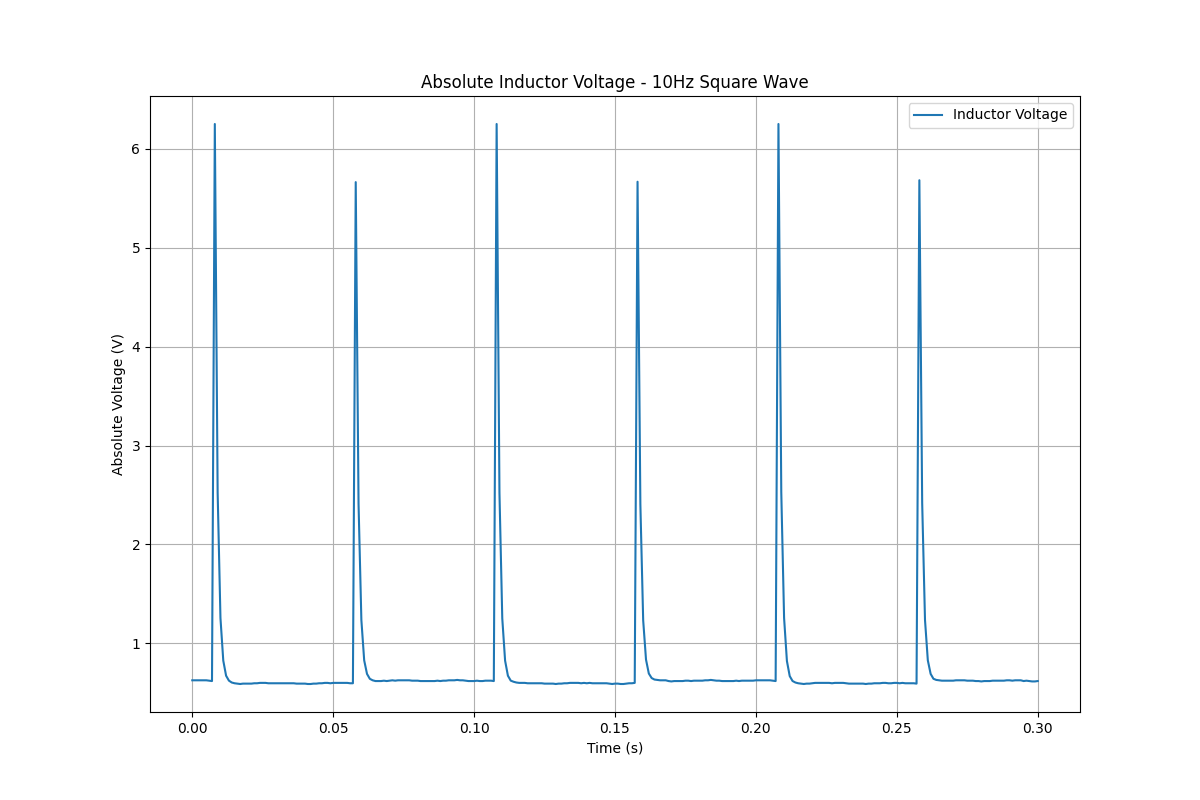
\includegraphics[width=5in]{images/abs_inductor_voltage_square.png}
    \caption{Absolute value of inductor voltage over time}
    \label{fig:square}
\end{figure}

\begin{figure}[ht]
    \centering
    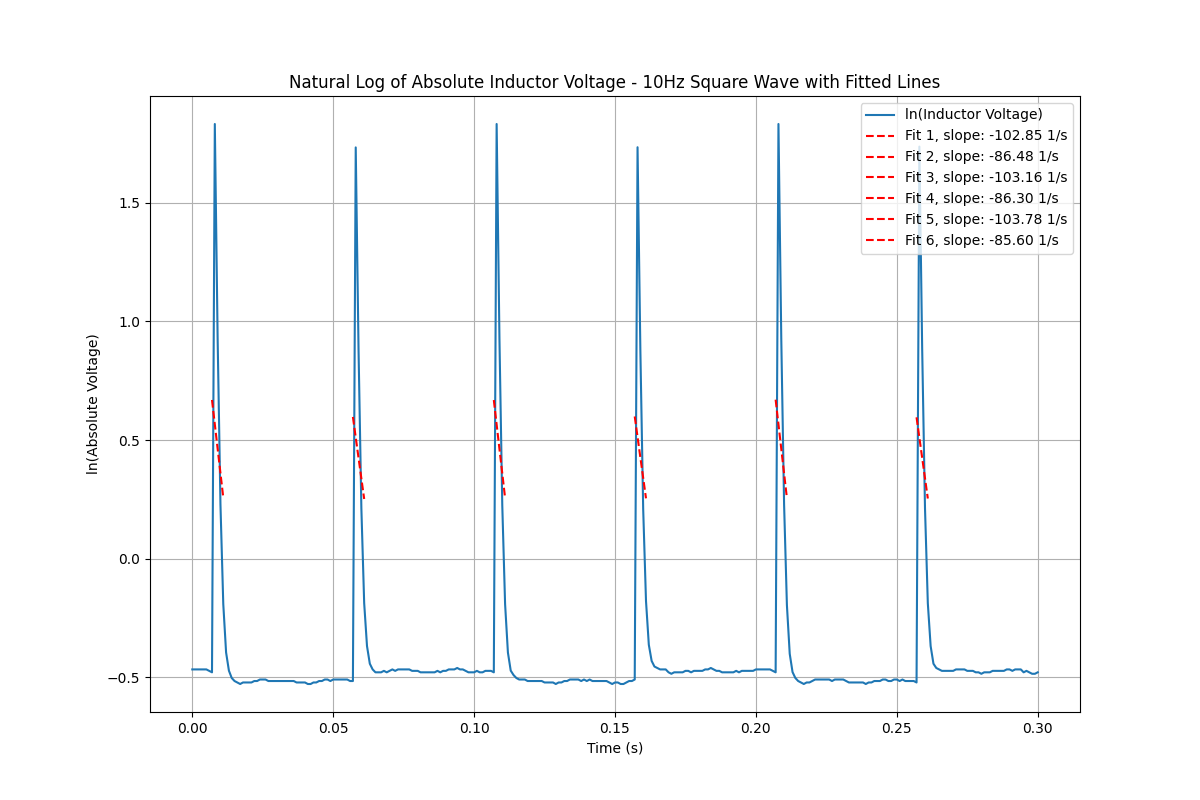
\includegraphics[width=5in]{images/ln_abs_inductor_voltage_square_with_fits.png}
    \caption{Natural log of inductor voltage with slopes fitted}
    \label{fig:square}
\end{figure}

\begin{table}[h]
\centering
\begin{tabular}{|c|c|c|}
\hline
Rise & Slope (1/s) & Inductance (H) \\
\hline
1 & -102.85 & 0.035974 ± 0.001033 \\
2 & -86.48 & 0.042785 ± 0.001258 \\
3 & -103.16 & 0.035868 ± 0.001030 \\
4 & -86.30 & 0.042876 ± 0.001261 \\
5 & -103.78 & 0.035653 ± 0.001023 \\
6 & -85.60 & 0.043226 ± 0.001273 \\
\hline
Average & -94.69 & 0.039397 ± 0.000470 \\
\hline
\end{tabular}
\caption{Slopes and Calculated Inductances}
\label{tab:inductances}
\end{table}


\section{Conclusion}

To conclude, I was able to use the attributes of inductors in an RL circuit to compute the self-inductance of the Helmholtz coil to be $\mathbf{0.039397 \pm 0.000470}\textbf{ Henries}$.


% \bibliographystyle{unsrtnat}
% \bibliography{references}

\end{document}
